\section{Application to proplyd bowshocks}
\label{sec:application}

Proplyds are comet-like structures observed in HII regions like Orion Nebula Cluster (ONC). 
These objects are interpreted as a D-type Ionization Front (IF) of a photoevaporated flow 
originated in the protoplanetary disk of a nearby low mass YSO \citep{Johnstone:1998}.
The pressure of the surrounding gas is not enough to confine this flow \citep{HA:1998}
may be formed by the interaction of the photoevaporated wind of the proplyds with the stellar wind of $\theta^1~C~Ori$, which is highly supersonic $(M \sim 100)$. 

The density distribution of the photoevaporated flow can be determined using the steady state continuity equation and assuming that almost all ionizing photons are absorbed at the IF \citep{HA:1998} and ignoring dust absorption, can be found that

\begin{align}
N(r_{IF},\theta) = N_0 \cos^{0.5}\theta
\label{eq:nprop}
\end{align}

This scenario can be described with the formalism of \citep{Canto:1996}, who proposes an algebraic solution for the two winds interaction problem in the thin shell approximation, in terms of a free parameter $\beta\equiv\frac{\dot{M}_wv_w}{\dot{M}_{w1}v_{w1}}$,
the winds momentum ratio, which the quantities with subindex 1 corresponds to the strongest wind, therefore $\beta<=1$. 

If we apply the \citep{Canto:1996} formalism for a photoevaporated flow with density given by (\ref{eq:nprop}), we find that the solutions for equations (8) - (11) of \citep{Canto:1996} are the following:

\begin{align}
\dot{M}_w &= \frac{\dot{M}_w^0}{3}\left(1-\cos^{3/2}\theta\right) \label{eq:dotprop} \\
\dot{\Pi}_z &= \frac{1}{5}v_w \dot{M}_w^0\left(1-\cos^{5/2}\theta\right)  \label{eq:pir}\\
\dot{\Pi}_r &= \frac{1}{2}v_w\dot{M}_w^0\left(\frac{4}{5}E\left(\frac{\theta}{2}|2\right) - \frac{1}{5}\sin 2\theta\cos^{1/2}\theta\right) \label{eq:piz}\\
\dot{J}_w = 0 \label{eq:jdot}
\end{align}  
The solution for (\ref{eq:piz}) includes an incomplete elliptic integral of the second kind. Combining equations  (\ref{eq:dotprop}) to (\ref{eq:jdot}) with equation (6) of \citep{Canto:1996}
numerically in python code, we can obtain the bow shock shape $R(\theta)$, as illustred in figure (\ref{fig:r-beta}).


% Combining equations (6),(9)-(11) and (19)-(23) from \citep{Canto:1996} and (\ref{eq:nprop}), we can solve numerically for $R(\theta)$, which gives us the shell's shape. Also we can
%obtain a relation between $\theta$ and $\theta_1$

%\begin{align}
%\theta_1\cot\theta_1 = 1+ 2\beta I(\theta)\cot\theta - \frac{4}{5}\beta\left(1-\cos^{5/2}\theta\right)
%\label{eq:th1th}
%\end{align}

%Where $I(\theta)\equiv \int^\theta_0 \cos^{1/2}\theta\sin^2\theta~d\theta$. The solution of this integral is an incomplete elliptical integral of the second kind:

%\begin{align}
%\int^\theta_0 \cos^{1/2}\theta\sin^2\theta~d\theta = \frac{4}{5}E\left(\frac{\theta}{2}|2\right) - \frac{1}{5}\sin 2\theta\cos^{1/2}\theta
%\end{align}

\begin{figure}
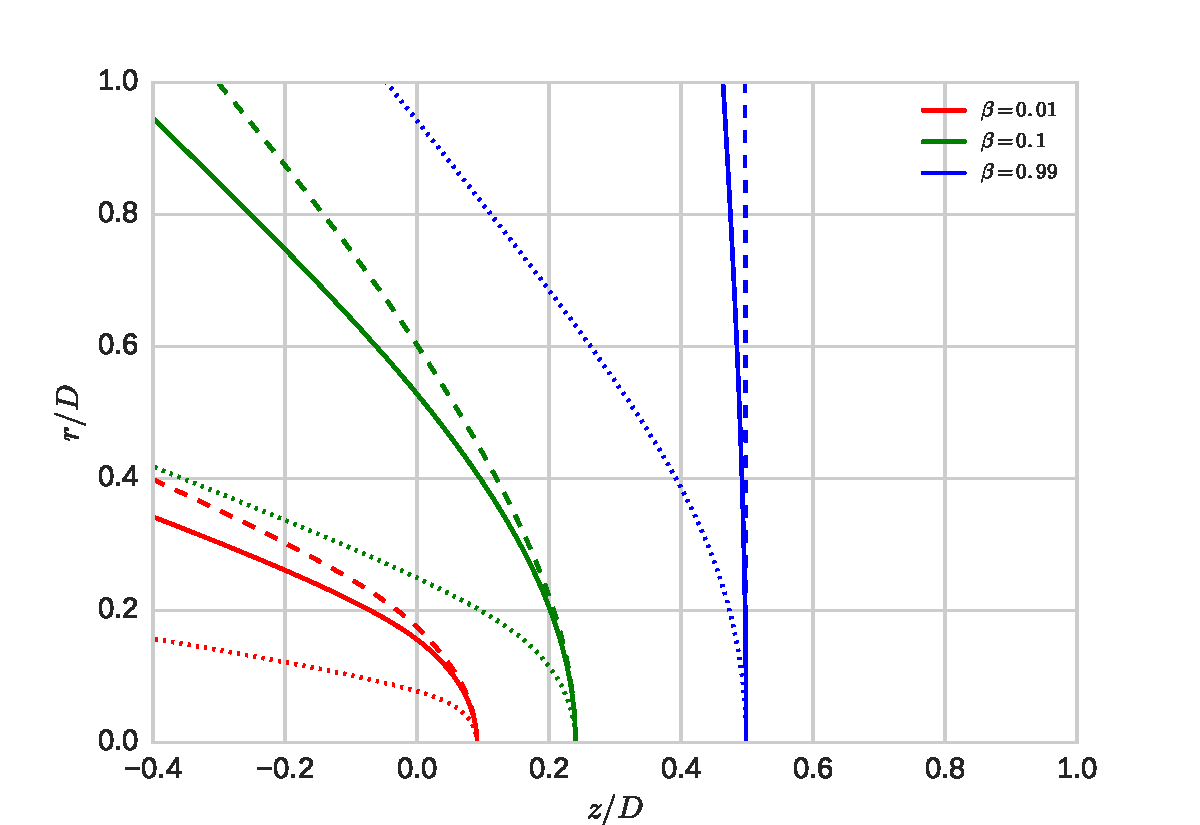
\includegraphics[width=\linewidth]{r-beta}
\caption{Bow shock shapes obtained with the \citep{Canto:1996} algebraic formalism using (\ref{eq:nprop}) to describe the proplyd wind density. The distance are normalized with $D$
to avoid dependency with this parameter.}
\label{fig:r-beta}
\end{figure}

\subsection{Characteristic Radii}

In order to find an analytic form of the characteristic radii $(R_0,R_c,R_{90})$, we may combine equations (\ref{eq:dotprop}) to (\ref{eq:jdot}) with (6) and (23) from \citep{Canto:1996}
and obtain the following relation:


\begin{align}
\theta_1\cot\theta_1 -1 =  \frac{8}{5}\beta E\left(\frac{\theta}{2}|2\right)\cot\theta - \frac{4}{5}\beta
\label{eq:th1th}
\end{align}

$R_0$ is obtained directly from equation (27) of \citep{Canto:1996} as the distance from the inner source where the RAM pressure of the interacting winds is in equilibrium.

We can obtain $R_{90}$ by the following process:
Evaluating equations  (\ref{eq:th1th}) and (23) from \citep{Canto:1996} at $\theta=\frac{\pi}{2}$ we obtain the following:

\begin{align}
R_{90} &= D\tan\theta_{1,90} \\
\theta_{1,90}\cot\theta_{1,90} &= 1-\frac{4}{5}\beta \label{eq:th190}
\end{align}
Where $\theta_{1,90}\equiv \theta_�(\frac{\pi}{2})$. Combining both equations we have:

\begin{align}
R_{90} &= D\frac{\theta_{1,90}}{1-\frac{4}{5}\beta} 
\end{align}

Expanding (\ref{eq:th190}) until 3rd order and solving for $\theta_{1,90}$:
\begin{align}
\theta_{1,90} \simeq \left(\frac{2.4\beta}{1-0.8\beta}\right)^{1/2} \\
R_{90} \simeq \left(\frac{2.4\beta}{(1-0.8\beta)^3}\right)^{1/2}
\label{eq:r90}
\end{align}
%%%% Here we go in edition

Now, to obtaining $R_c$ we expand  (\ref{eq:th1th}) until order 2nd order for small $\theta$ values to find that for such values
$\theta_1 = \beta^{1/2}\theta$

Expanding equation (23) from \citep{Canto:1996} and substituting $\theta_1$ we found that:

\begin{align}
R \simeq R_0 \left(1+\frac{1+2\beta^{1/2}}{6}\theta^2\right)
\label{eq:R_approx}
\end{align}

Which lead us to derive the radius of curvature at the symmetry axis:

\begin{equation}
R_c = \frac{3}{2}R_0\left(1-\beta^{1/2}\right)^{-1}
\label{eq:Rcurv}
\end{equation}

Equations (\ref{eq:r90}),  (\ref{eq:Rcurv}) and (27) from \citep{Canto:1996} are labeled as ``analytic i=0'' in figure (\ref{fig:rad-beta}).

\begin{figure*}
\begin{tabular}{ccc}
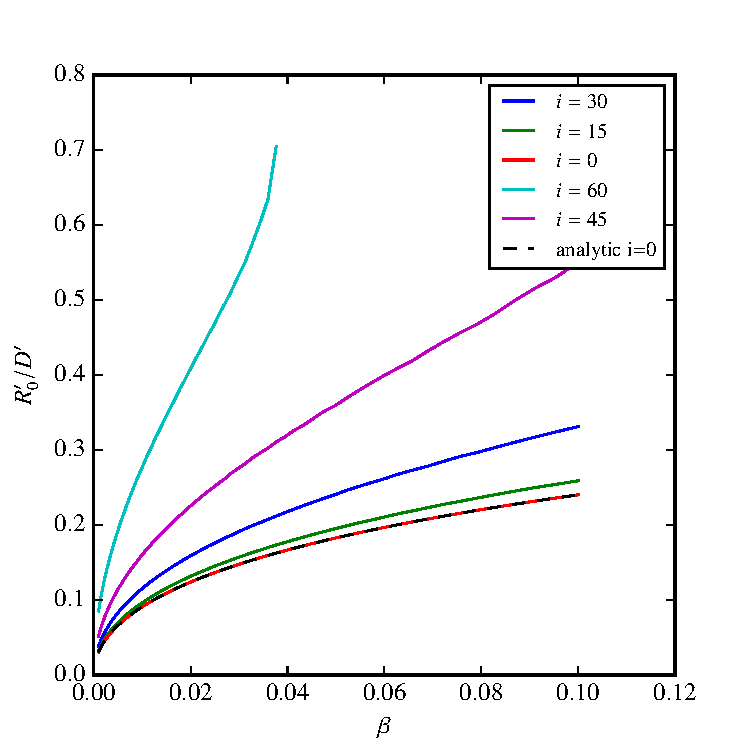
\includegraphics[width=0.35\linewidth]{R0-b}&
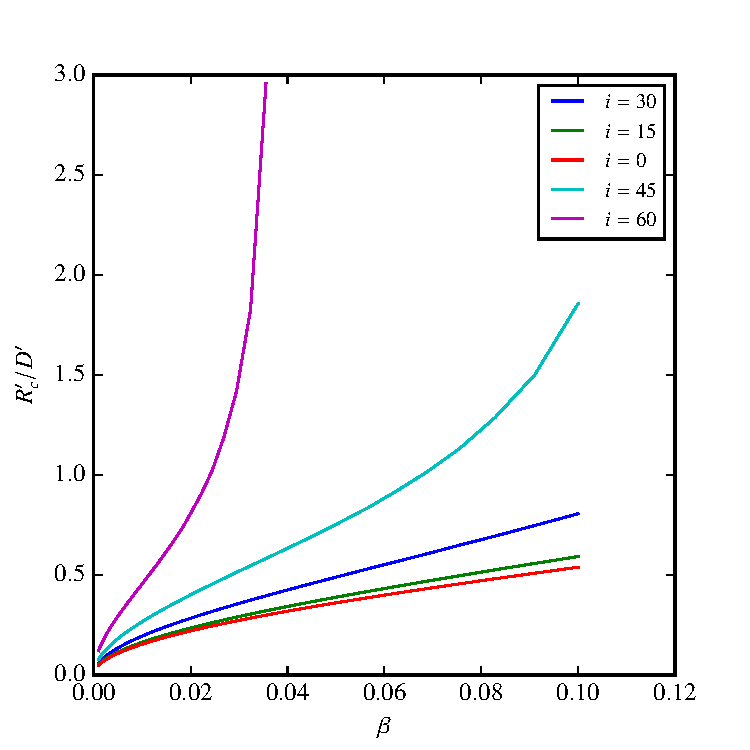
\includegraphics[width=0.35\linewidth]{Rc-b} &
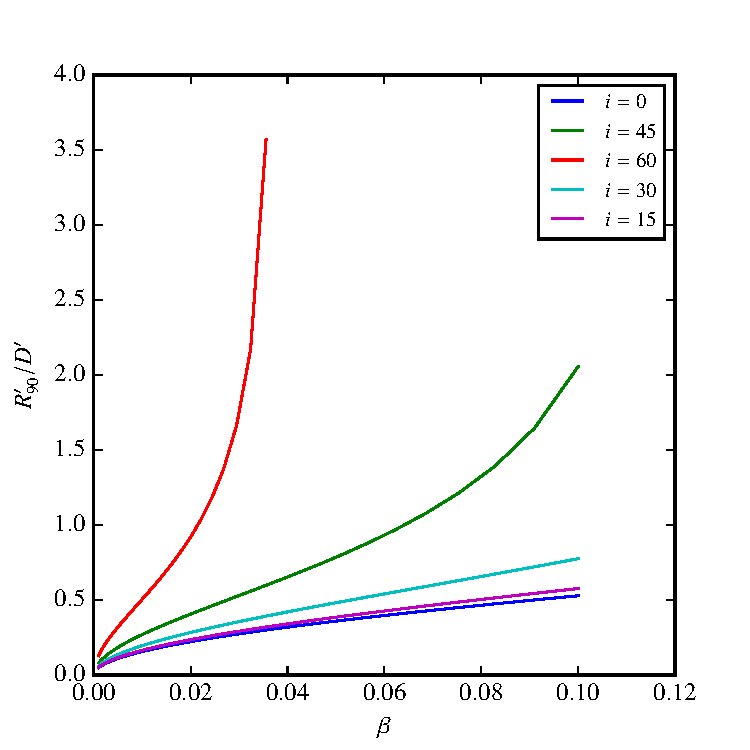
\includegraphics[width=0.35\linewidth]{R90-b}
\end{tabular}
\caption{$R_0$, $R_c$ and $R_{90}$ versus $\beta$ for a fixed set of inclinations. Equations (\ref{eq:r90}), (\ref{eq:Rcurv}), and (27) from \citep{Canto:1996}
are labeled as ``analytic i=0''. Note that the analytic solution deviates from the numeric solution when $\beta \gtrsim 0.1$}
\label{fig:rad-beta}
\end{figure*}

Observationally, we can measure the projected radii. In order to estimate the model parameters is neccesary to measure at least two of the mentioned radii, being $R_0$ the
easiest to measure. Therefore, we may compare both $R_c$ and $R_{90}$ against $R_0$ as shown in figure %(\ref{fig:radii-r0})

\subsection{Observational work}

We measured the Characteristic radii in Orion Nebula proplyds from observations with the ACS camera from the Hubble Space Telescope (HST) using a lamp filter around $\lambda = 5007 \AA$. The proposal for these observations were done by  Jogee, S. in 2004 with calibration purposes but (he never published anything using explicitly these observations). % We must check if this phrase should be included
Nevertheless, as we are only interested in measure the geometric shape of bow shocks, these observations are more than enough.

\subsubsection{Metodology}
Using the DS9 SAO image tools, we marked the positions of the proplyds and $\theta_1^C$. We followed the brightness contours along the 
bow shocks to mark the shell's position. In order to obtain the set of measurements $(R_0, R_c, D)$, we moved to the proplyd's reference frame, (where the proplyd's position)
is $(0,0)$ and measured distances in arcseconds. In this reference, the proplyd-$\theta_1^C$ line is $y=0$. With the shell's positions, we optimize a circle, whose radius is $R_c$, but
this optimization has two variants: the first one with the restriction that the center of the circle must lie in the symmetry axis (y=0), and the second variation is with no restrictions. The figure (\ref{fig:radii-measures-example}) shows a representation of the metodology described. 
Our first goal was comparing measurements of $(R_0,R_{90})$ of the LV group of proplyds in mid infrared by \citep{Robberto:2005} against observations in [OIII] with better angular resolution but less contrast against
the background.
In \citep{Robberto:2005} they compare their observations with shells obtained with the \citep{Canto:1996} two winds interactions formalism. They found no concordance between the model and observations. We attempted to redo the measurements with better resolution observations. We found quickly that we cannot measure $R_{90}$ in a reliable way since the shell's brightness decays toward the wings. Also, we are using a more sophisticated model where the proplyd's wind density decays as $n \propto \cos {1/2}\theta$ instead of an isotropic wind.
A better replacement of $R_{90}$ is the radius of curvature, defined as the radius of the circle that fits the observations, because always is measurable. Figures (\ref{fig:char-radii-obs}) and (\ref{fig:char-radii-obs-2}) show our measurements of the radius of curvature for the LV group, with exception of LV1, which actually is a binary proplyd, thus our model is not adequate in this case. Also we include the proplyds 167-328 and 177-341 (HST1) which are close enough to $\theta^1~\mathrm{C~Ori}$ to be influenced by it stellar wind.
Our results show a better concordance (but still not perfect) between models and observations, as shown in figure (\ref{fig:prop-shell-err}). A possible cause of the discrepancy may be that the \citep{Canto:1996} model assumes that the interacting winds are hypersonic in such way that the shocked gas can be considered as a bidimensional surface. In practice, the bow shock has a finite width, which can afect the apparent shape due to projection effects


\begin{figure*}
\begin{tabular}{cc}
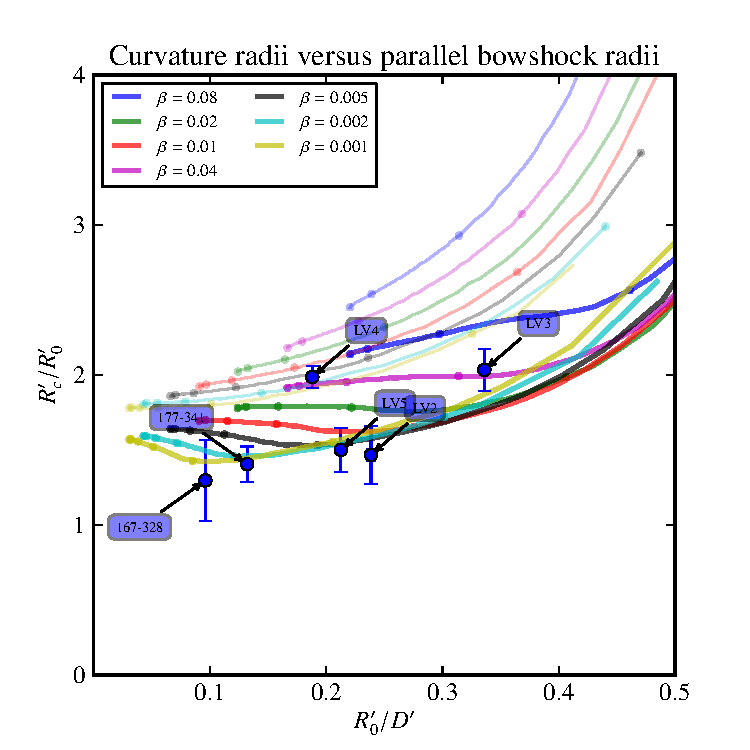
\includegraphics[width=0.45\linewidth]{proplyd-shell-R0-Rc-errors-1} &
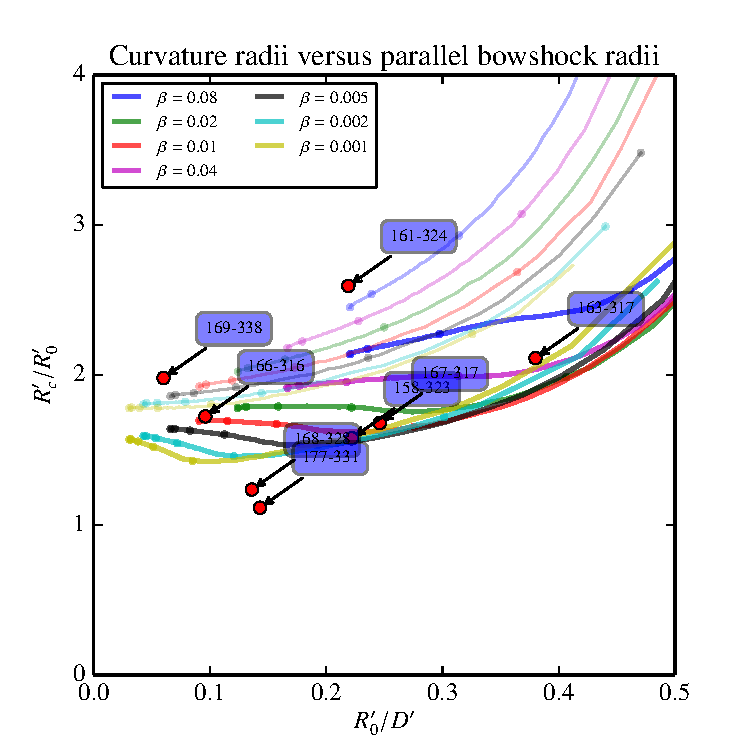
\includegraphics[width=0.45\linewidth]{proplyd-shell-R0-Rc-new}
\end{tabular}
\label{fig:prop-shell-err}
\caption{Measurements of proplyd's characteristic radii $R_c$ and $R_0$. The curves represent a single bow shock with  fixed wind's momentum ratio $\beta$. The dots represent separations in inclination of $15^{\circ}$. The semitransparent curves represent bow shocks which the inner wind is isotropic and the full colored curves bow shocks which inner wind density decays as $\cos^{1/2}\theta$. Our measures match far better than \citep{Robberto:2005}, but our data tend to lie at high inclinations $i \gtrsim 45^\circ$, when we expected the opposite. Right side: The same}
\end{figure*}
%Initially we tried to measure the radii $(R_0,R_{90})$, but it wasn't possible due to the fact that the brightness of the shell decays rapidly towards the wings, and using $R_\theta$ where $60 \lesssim \theta < 0 $ is not so useful, because there is not a significant difference between $R_0$ and $R_\theta$. Instead, we introduced the radius of curvature after we realized how well the shell's marks fits into a circle for all the proplyds (see figure (\ref{fig:char-radii-obs})).

\begin{figure*}
\begin{tabular}{cc}
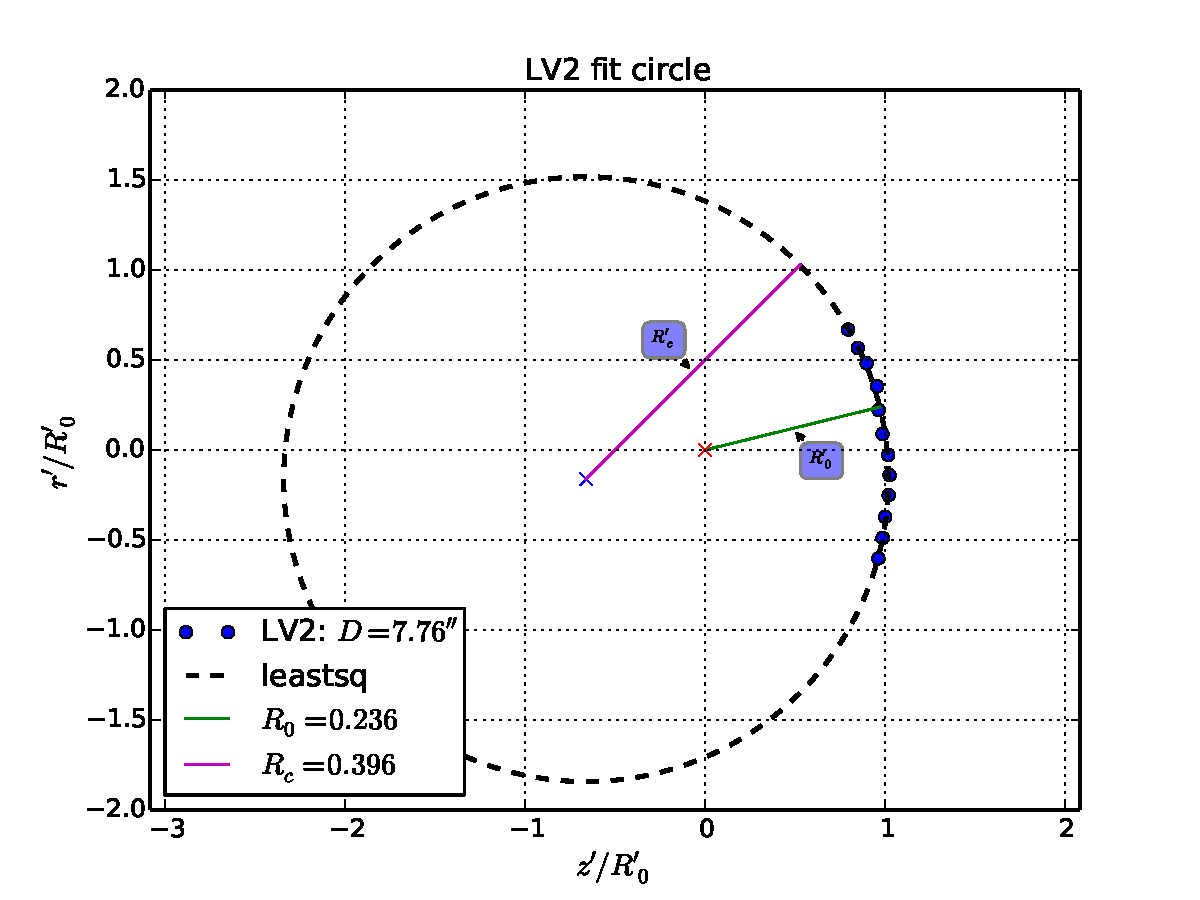
\includegraphics[width=0.5\linewidth]{LV-bowshocks-xyfancy-502epositions-LV2} & 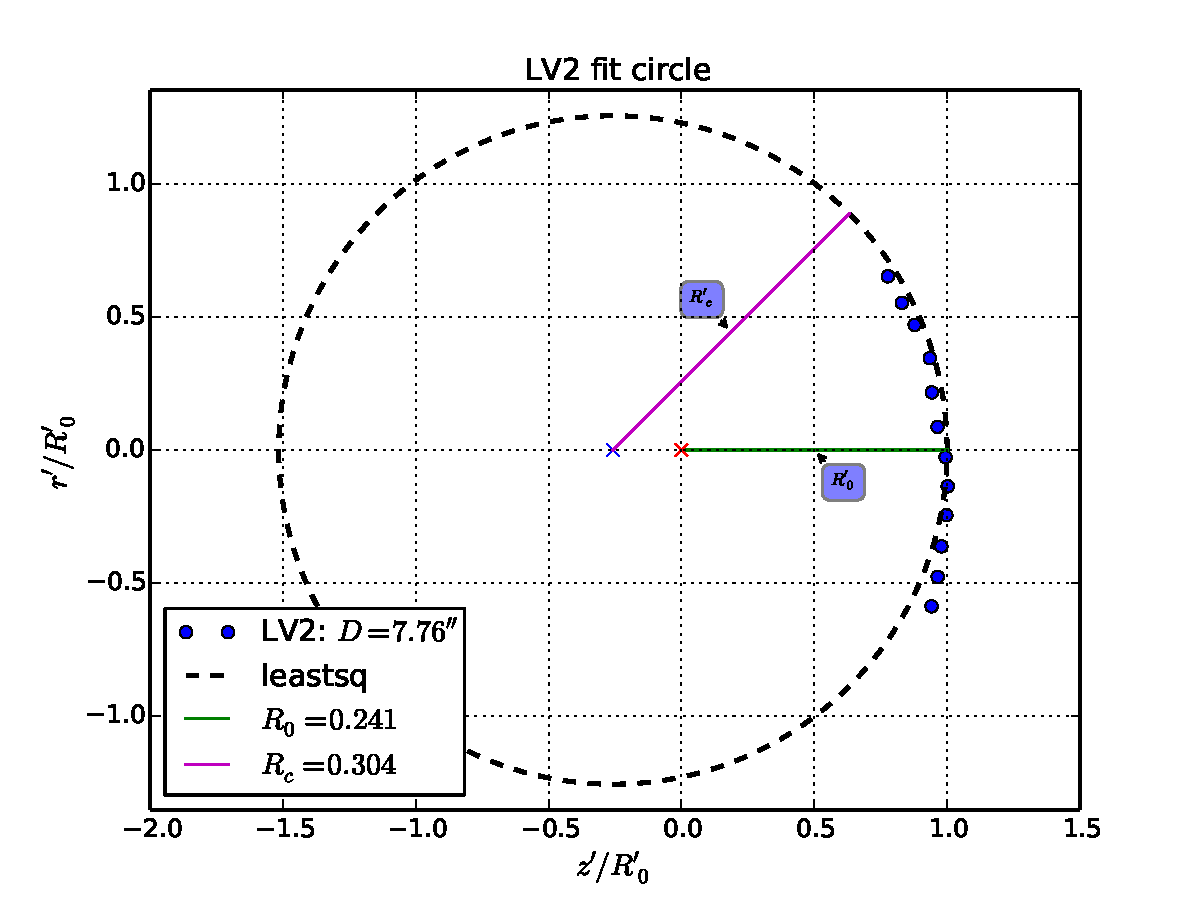
\includegraphics[width=0.5\linewidth]{LV-bowshocks-xyfancy-onaxis-502epositions-LV2} \\
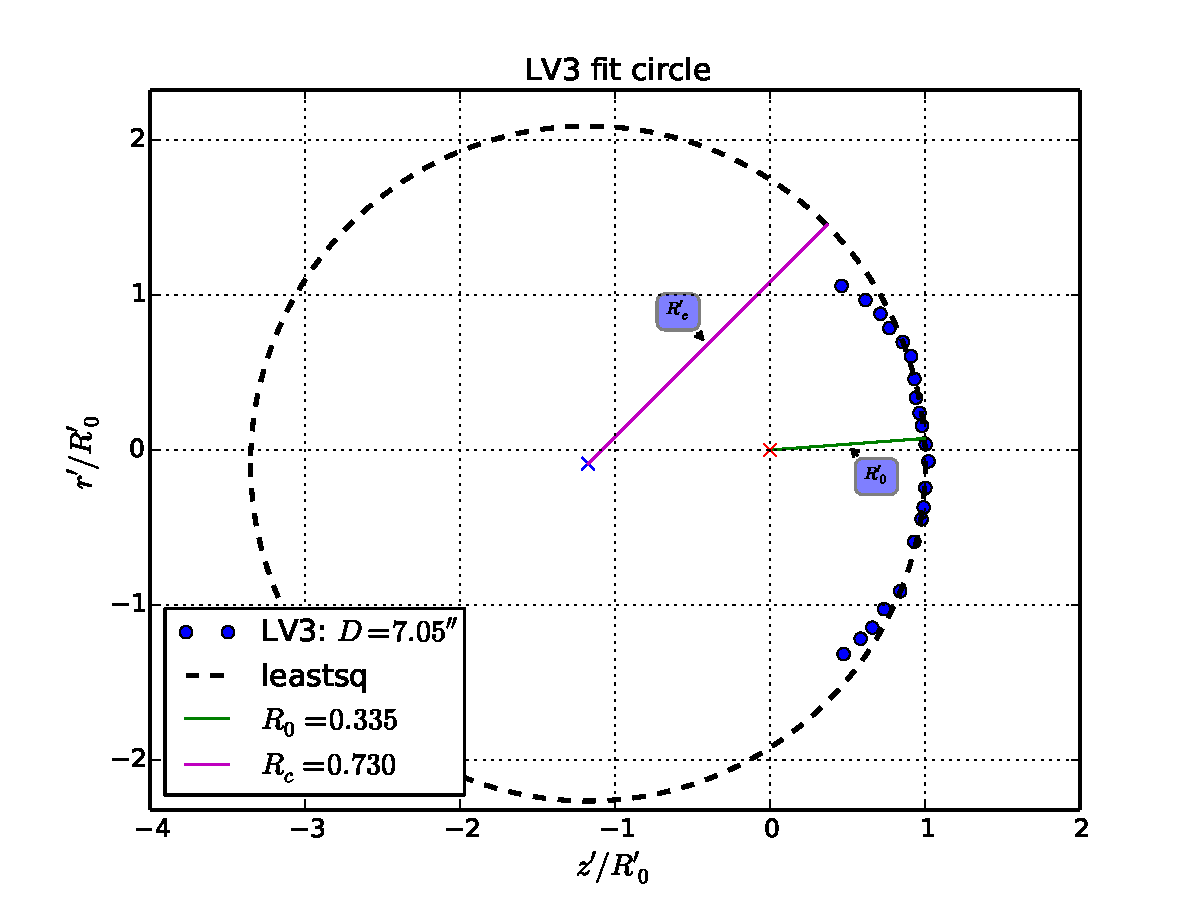
\includegraphics[width=0.5\linewidth]{LV-bowshocks-xyfancy-OIII3a-LV3} & 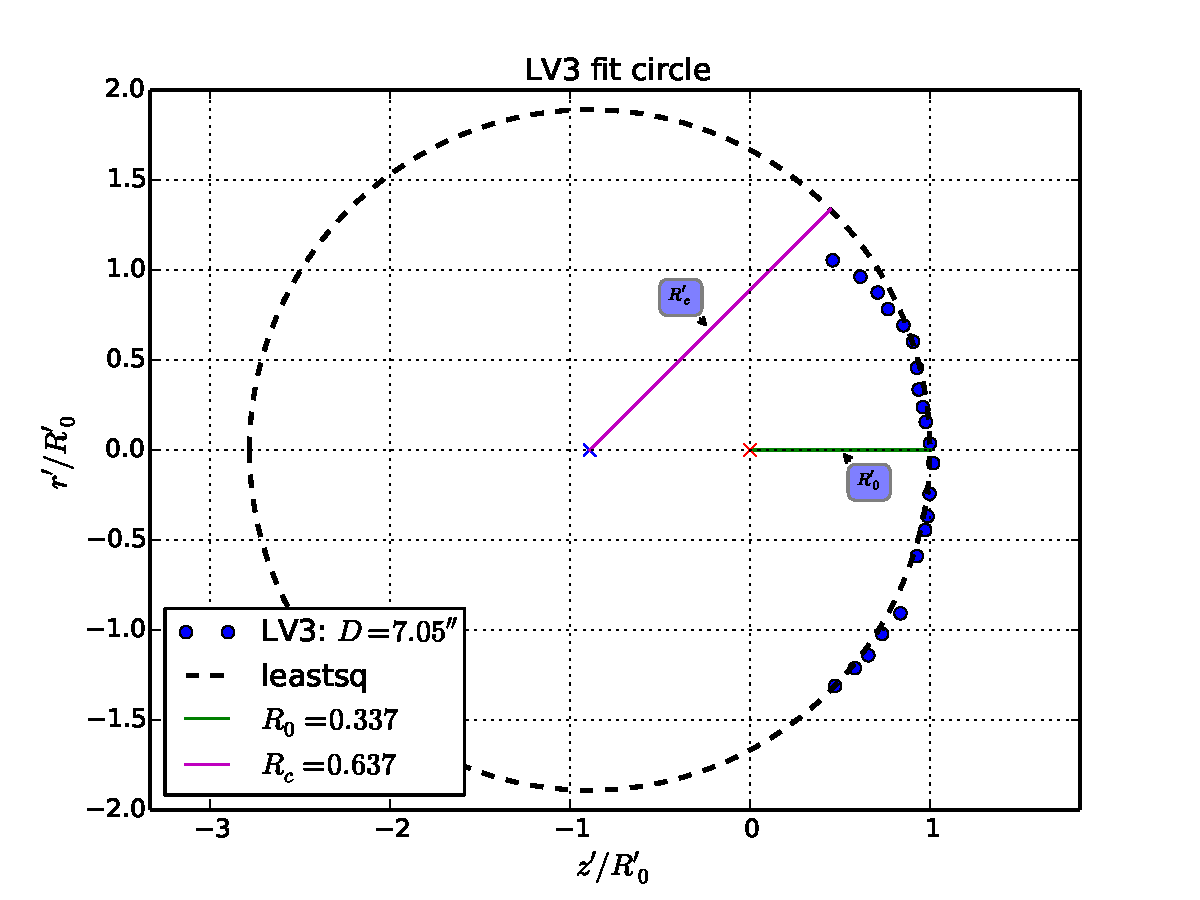
\includegraphics[width=0.5\linewidth]{LV-bowshocks-xyfancy-onaxis-OIII3a-LV3} \\
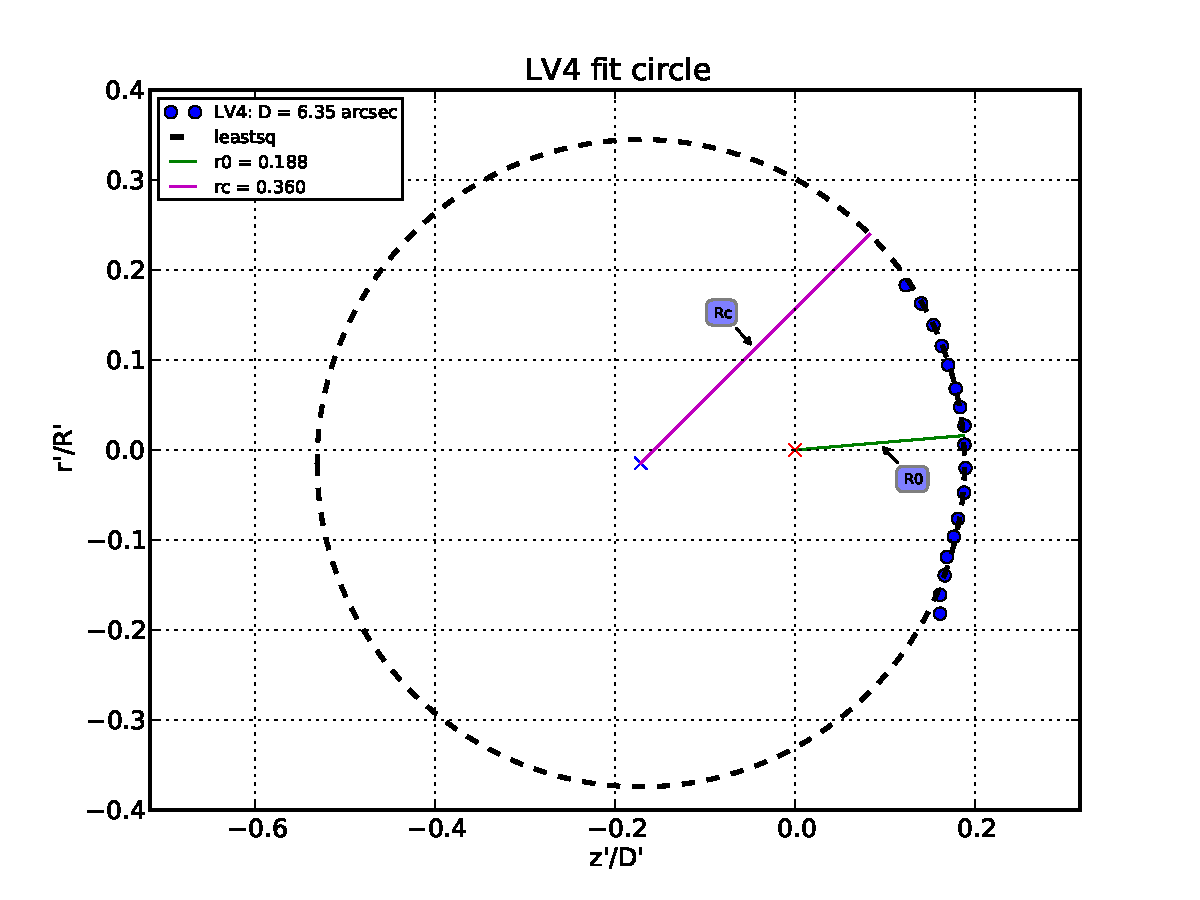
\includegraphics[width=0.5\linewidth]{LV-bowshocks-xyfancy-OIII3a-LV4} & 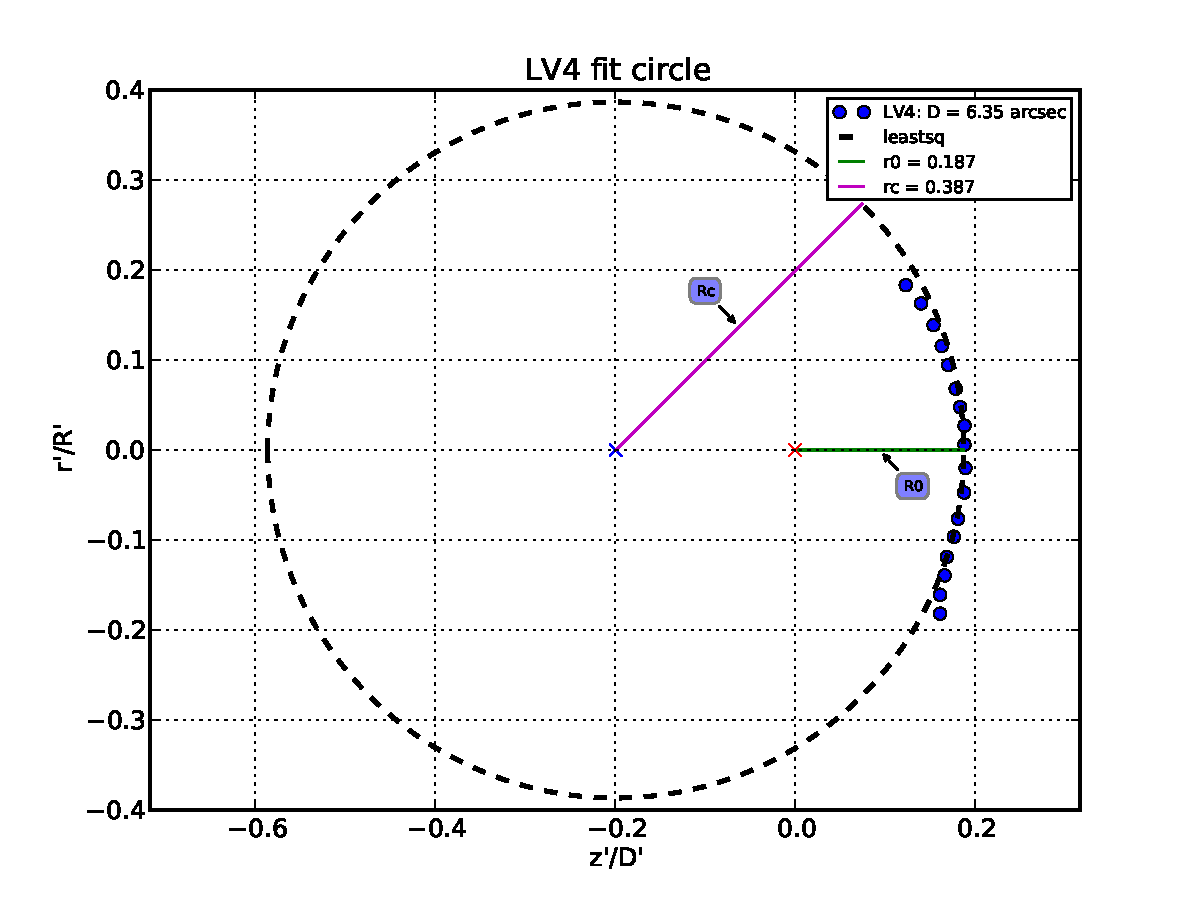
\includegraphics[width=0.5\linewidth]{LV-bowshocks-xyfancy-onaxis-OIII3a-LV4}
\end{tabular}
\label{fig:char-radii-obs}
\caption{Fits to the shell's shapes. In the left side we have the fits without any restrictions. In the right side we have the fits restricting the center of the circle to be in $y=0$. This data is summarized in table (\ref{tab:proplyds})}
\end{figure*}

\begin{figure*}
\begin{tabular}{cc}
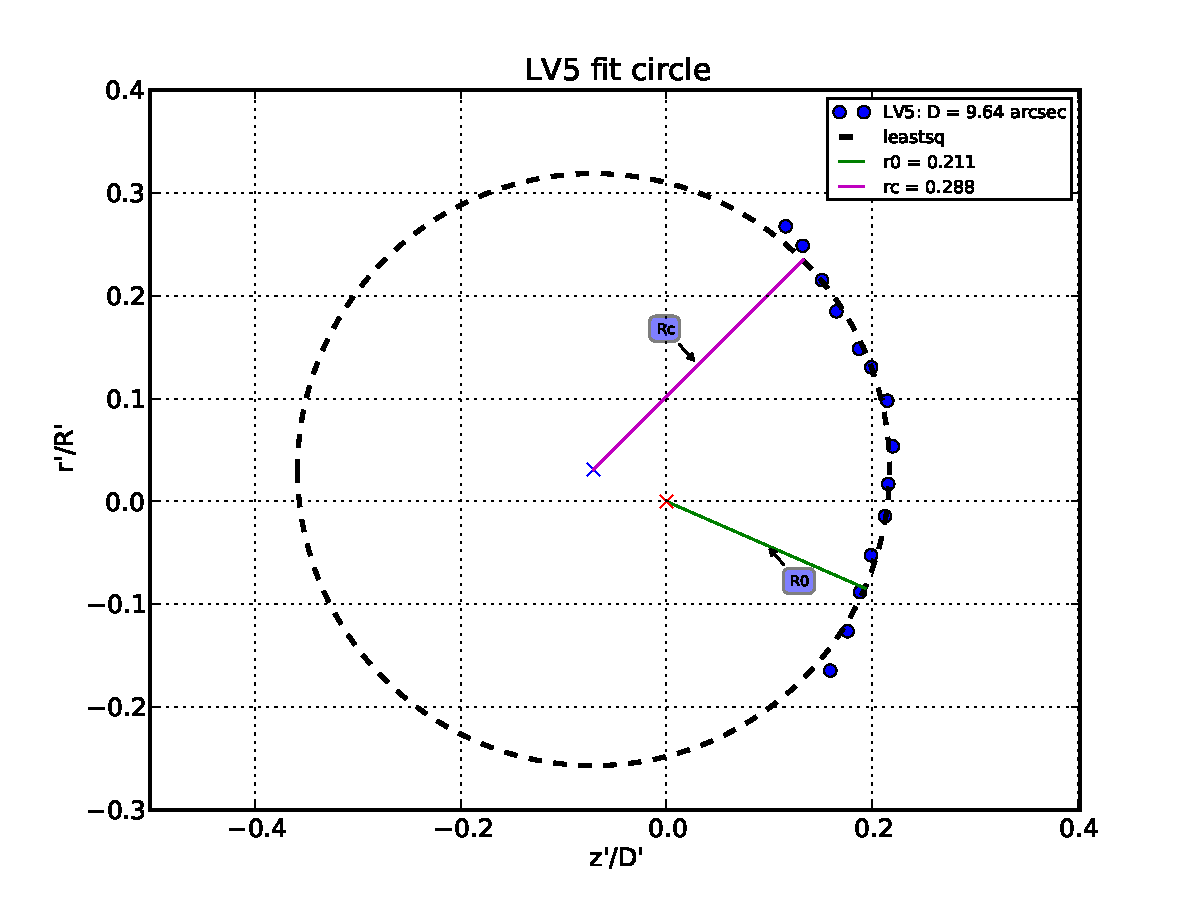
\includegraphics[width=0.5\linewidth]{LV-bowshocks-xyfancy-OIII3a-LV5} & 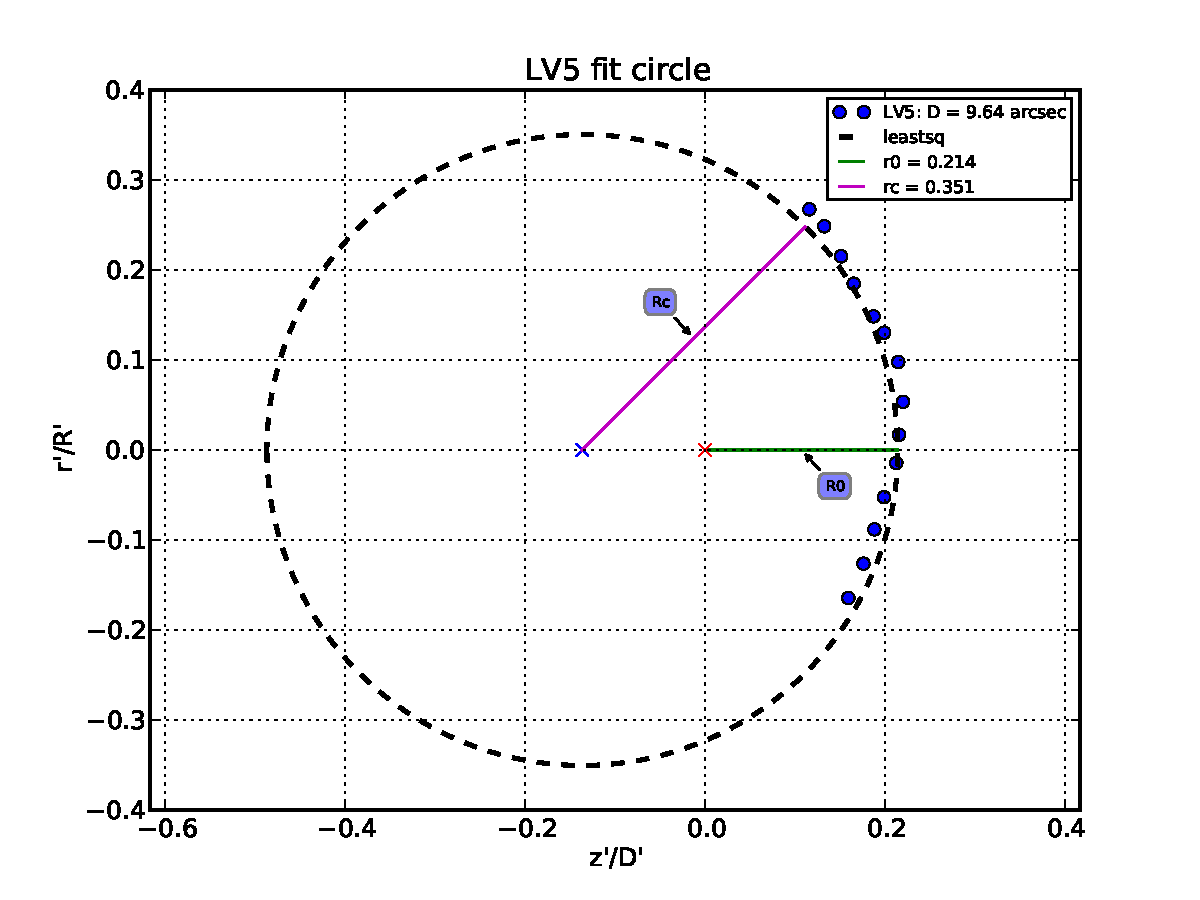
\includegraphics[width=0.5\linewidth]{LV-bowshocks-xyfancy-onaxis-OIII3a-LV5} \\
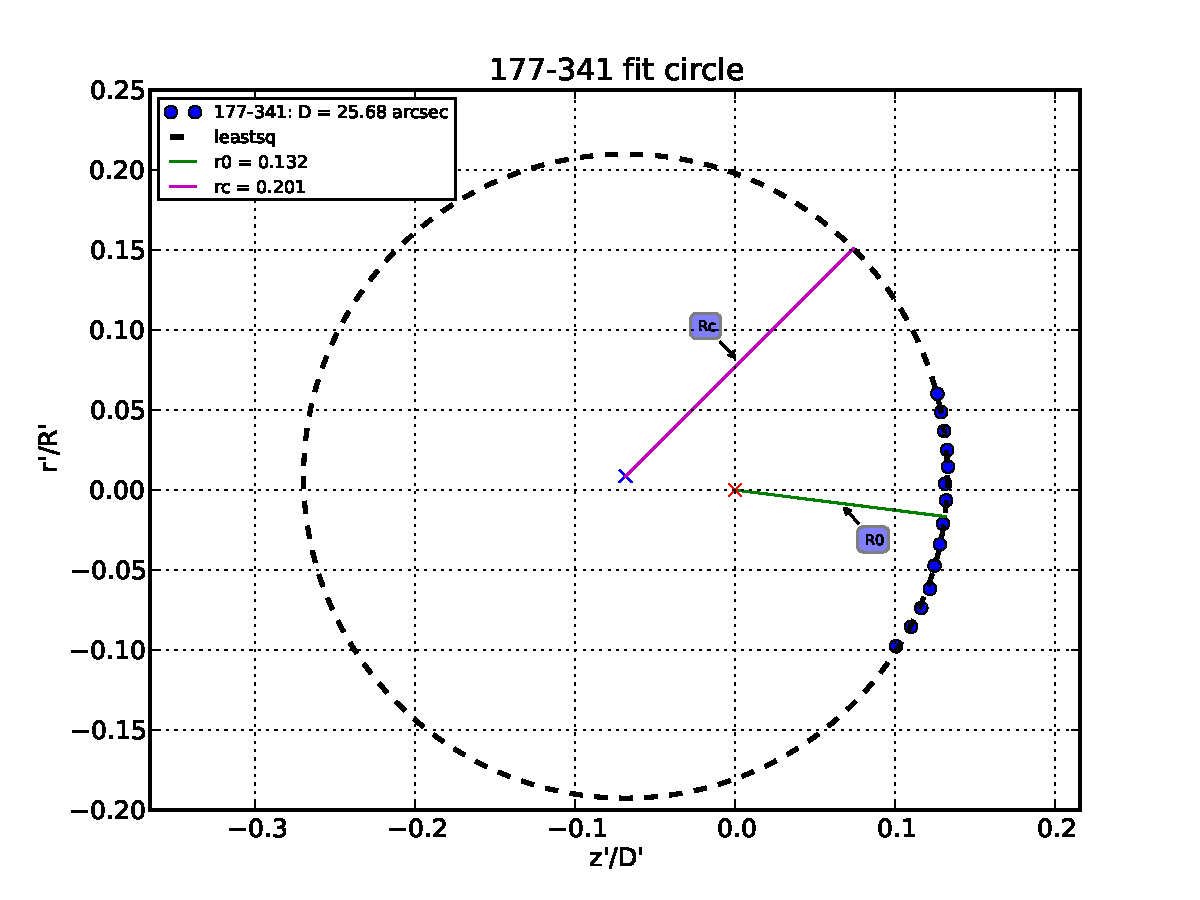
\includegraphics[width=0.5\linewidth]{LV-bowshocks-xyfancy-502epositions-177-341} & 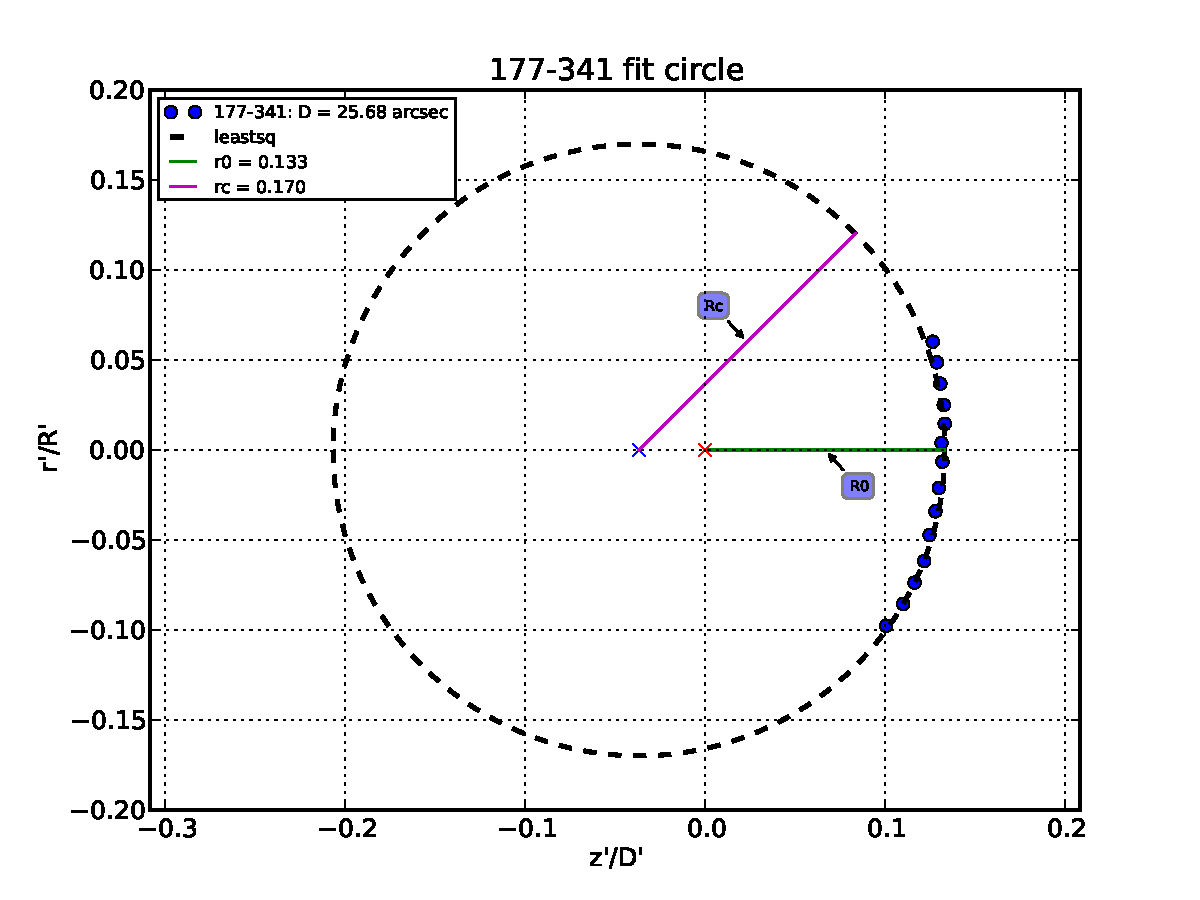
\includegraphics[width=0.5\linewidth]{LV-bowshocks-xyfancy-onaxis-502epositions-177-341}\\
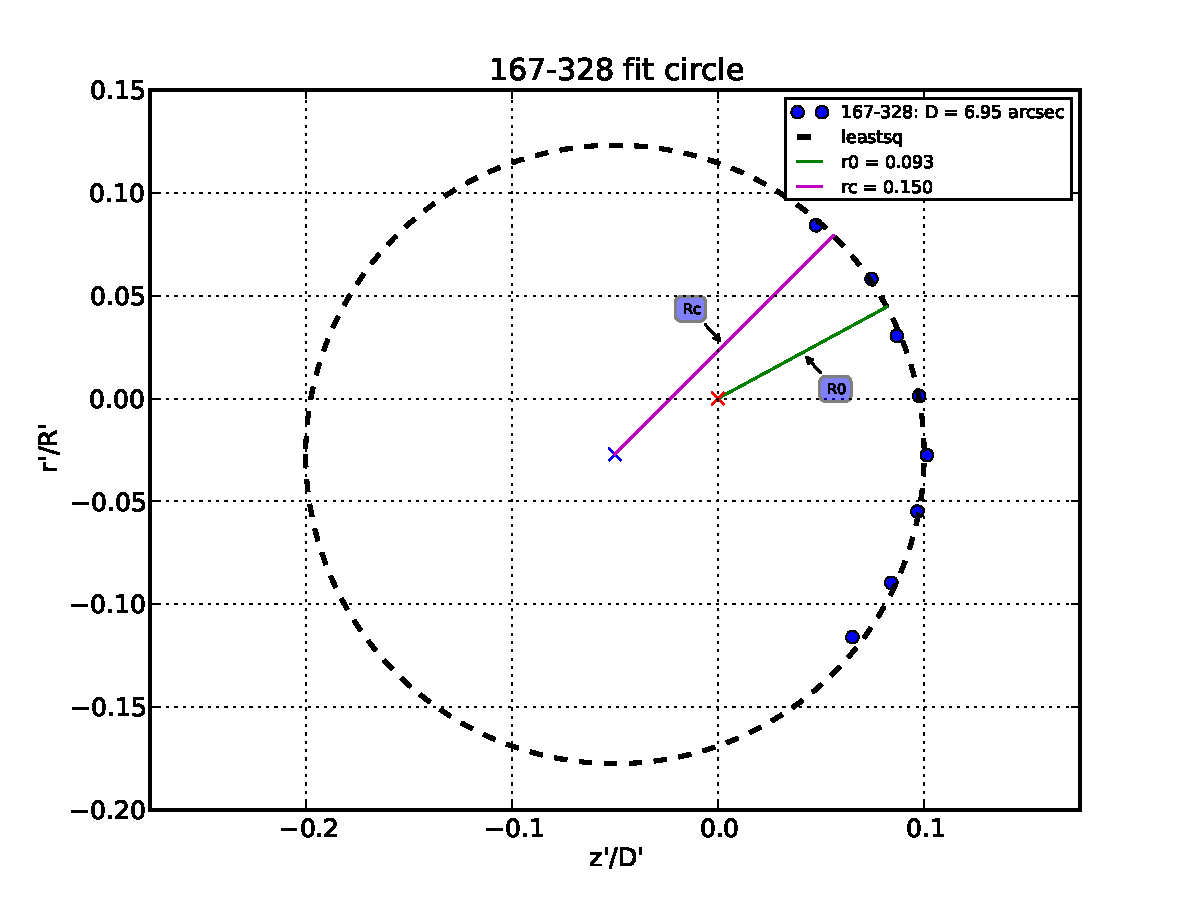
\includegraphics[width=0.5\linewidth]{LV-bowshocks-xyfancy-OIII3a-167-328} & 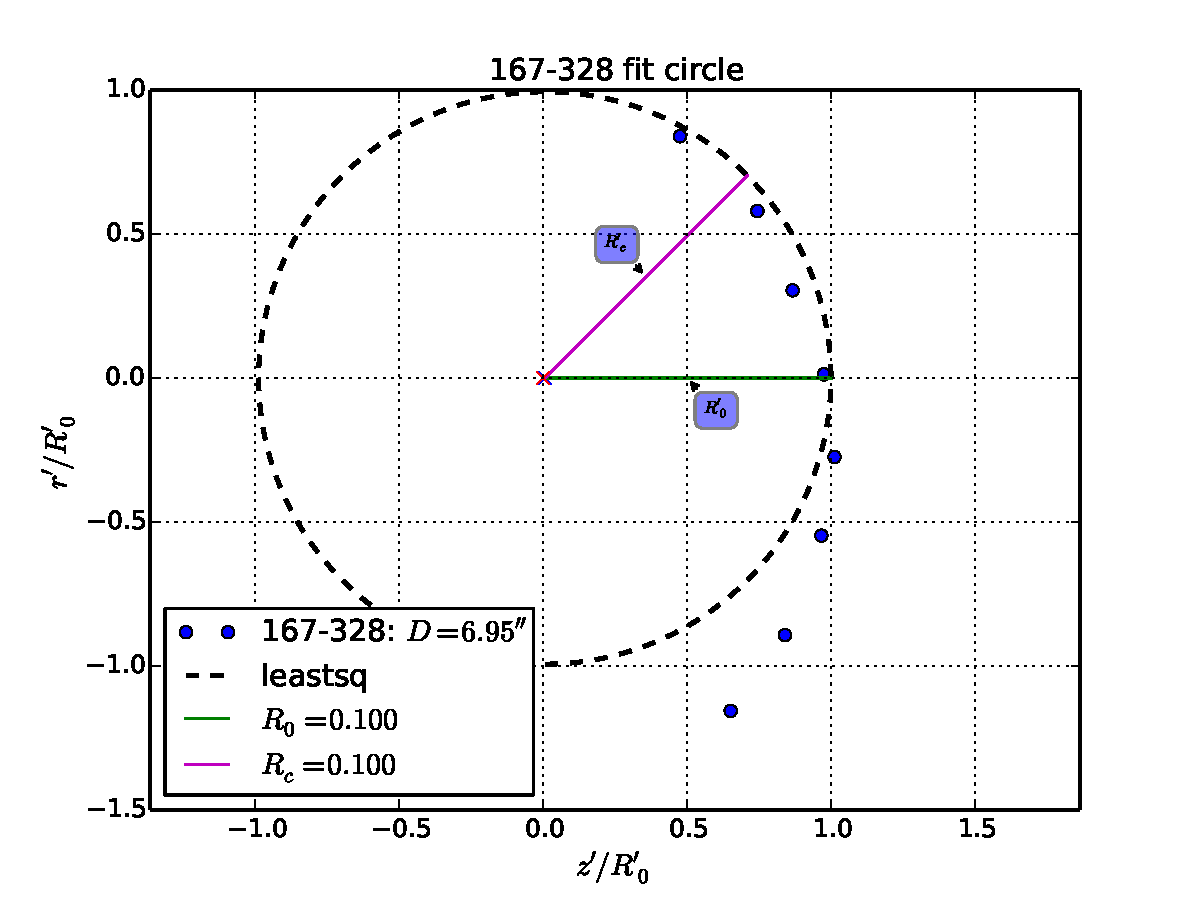
\includegraphics[width=0.5\linewidth]{LV-bowshocks-xyfancy-onaxis-OIII3a-167-328}
\end{tabular}
\label{fig:char-radii-obs-2}
\caption{Continuation of figure (\ref{fig:char-radii-obs})}
\end{figure*}


\begin{figure}
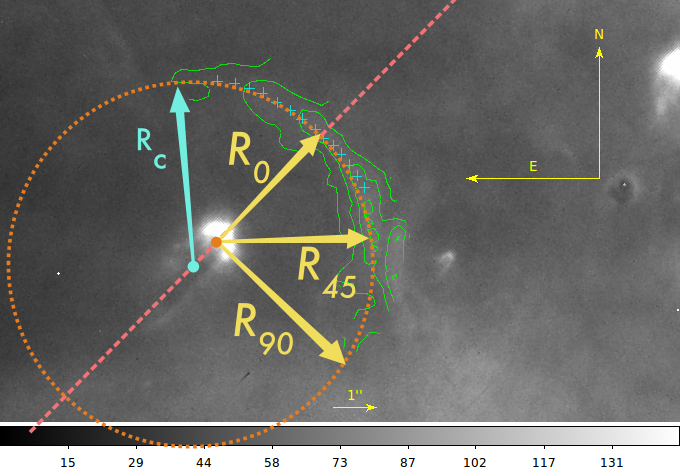
\includegraphics[width=\linewidth]{177-341-will-anota}
\caption{Schematic example of the observational measures used. We don't use $R_\theta$ any longer, but instead the radius of curvature}
\label{fig:radii-measures-example}
\end{figure}

 \begin{table*}
\begin{tabular}{c|ccccccccc}\hline
Proplyd & LV2 & LV2b & LV3 & LV4  & LV5 & 177-341 & 168-328 & 169-338 & 180-331\\\hline
$D (\arcsec)$ &7.76 & 7.21 &6.89 & 6.2 & 9.55 & 25.65 & 6.83 & 16.43 & 25.07 \\
$R_c/D$  & 0.23  & 0.19& 0.61  & 0.5  & 0.34  & 0.18  & 0.22 & 0.09 & 0.09\\
$R_0/D$  & 0.32 & 0.1 & 0.34 & 0.19 & 0.21 & 0.14 & 0.15 & 0.06 & 0.07\\
$R_c/R_0$ & 0.73 & 2.00 & 1.83 & 2.68  & 1.57 & 1.22 & 1.47 & 1.46 & 1.30  
\end{tabular}
\caption{Characteristic Radii measurements for a sample of proplyds. %Enhance description when more rows were included
} 

\label{tab:proplyds}
\end{table*}

%%% Local Variables:
%%% mode: latex
%%% TeX-master: "proplyd-bowshocks.tex"
%%% End:


%\begin{figure}
%\end{figure} 

%\begin{figure*}
%\begin{tabular}{cc}
%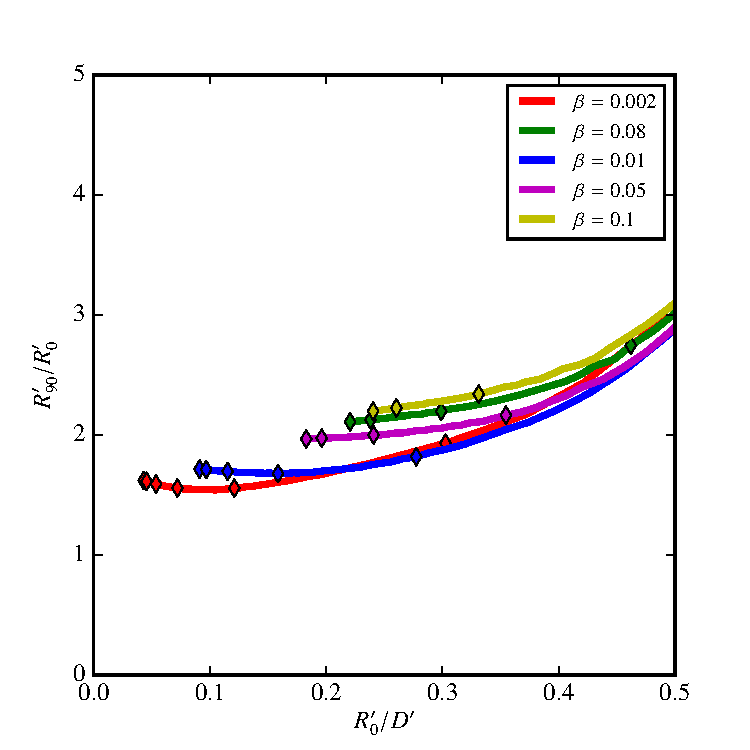
\includegraphics[width=0.5\linewidth]{R90-R0-b}&
%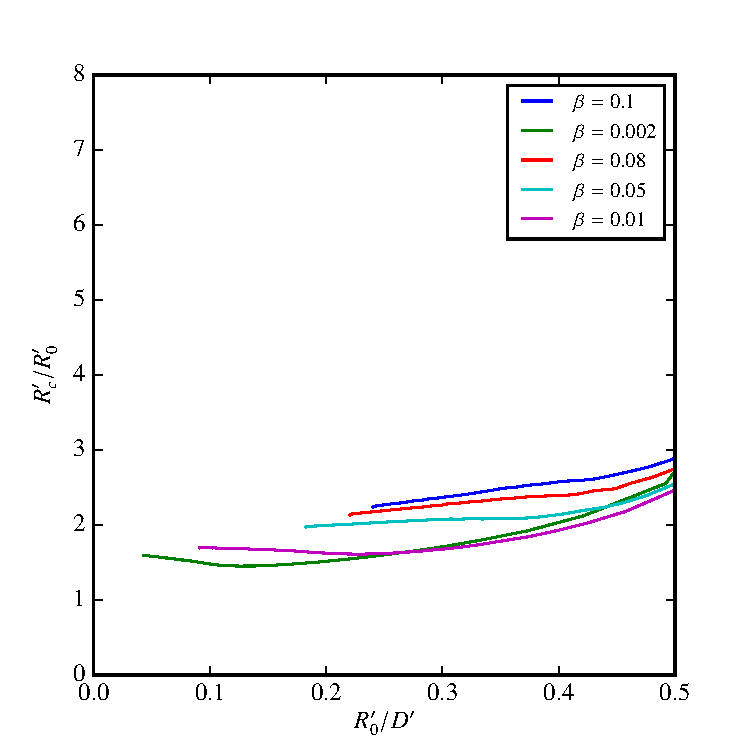
\includegraphics[width=0.5\linewidth]{Rc-R0-b}
%\end{tabular}
%\label{fig:radii-r0}
%\caption{Left: $R_c$ normalized with $R_0$ vs $R_0$ normalized with $D$. Right:$R_{90}$ normalized with $R_0$ vs $R_0$ normalized with $D$. Since the bow shock brightness decays 
%at the wings, it is more difficult to measure $R_{90}$. Along every single curve, $\beta$ is constant. The marks in the curves represents jumps of $15^\circ$ in inclination, and the most left 
%mark in each curve represent $i=0^\circ$}
%\end{figure*}


%%% Local Variables:
%%% mode: latex
%%% TeX-master: "proplyd-bowshocks"
%%% End:
